
\section*{Cycle 1}

\section{\Large{Basics of Network Configurations Files and Networking \\Commands in Linux}}

\subsection{Aim}
\large To get started with the basics of network configurations, files and networking
commands in Linux.

\subsection{Theory \& Output}
\Large{Basic Commands :}
\begin{itemize}
    \item ifconfig
        \begin{itemize}
            \item Stands for ”interface configuation”. 
            \item Used to initialize an interface, assign IP address to interface and enable or disable interface on demand.
            \item With this command you can view IP Address and Hardware / MAC address assign to interface and also MTU(Maximum transmission unit) size.
        \end{itemize}
        \begin{figure}[h]
            \centering
            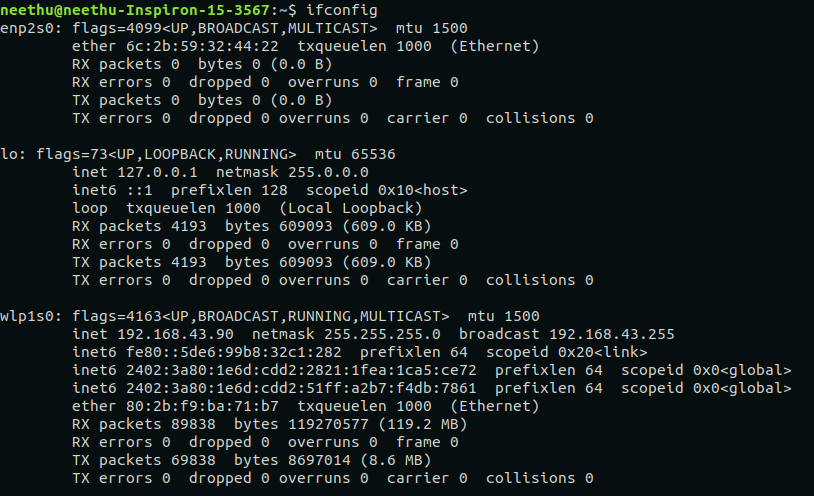
\includegraphics[scale=0.6]{img/e11.png}
        \end{figure}
    \item ping
        \begin{itemize}
            \item It is used to test the connectivity of a network considered.
            \item It uses the ICMP (Internet Control Message Protocol) and sends a series of ICMP echo request messages to the target host and waits for an ICMP echo reply.
            \item It helps to calculate the package loss, round trip time of the packets, and whether the target host is reachable.
        \end{itemize} 
        \begin{figure}[h]
            \centering
            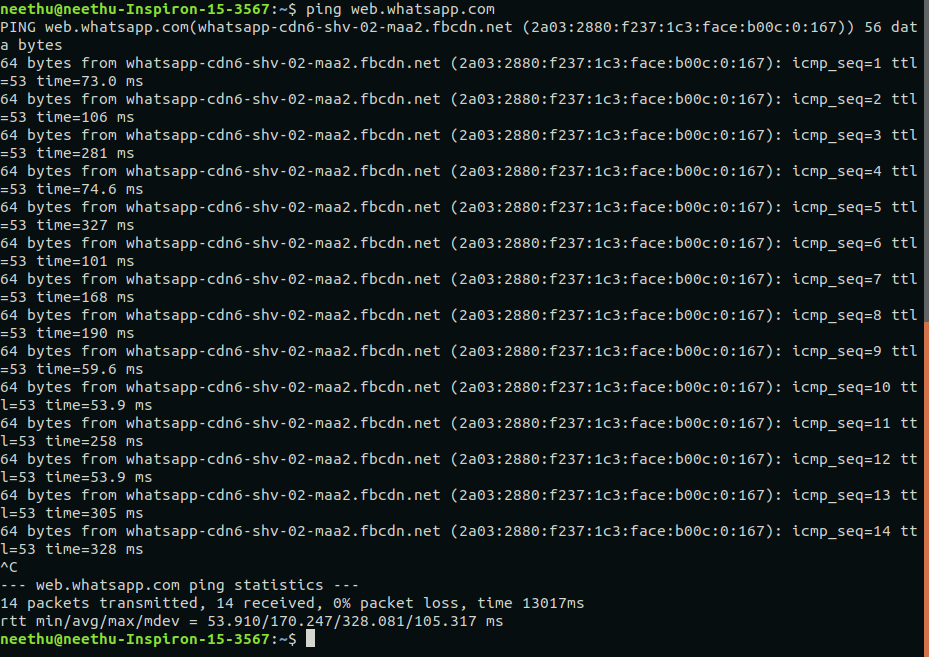
\includegraphics[scale=0.5]{img/e12.png}
        \end{figure}
    \item traceroute
        \begin{itemize}
            \item It is a network troubleshooting utility which shows number of hops taken to reach destination also determine packets traveling path.
        \end{itemize}
        \begin{figure}[h]
            \centering
            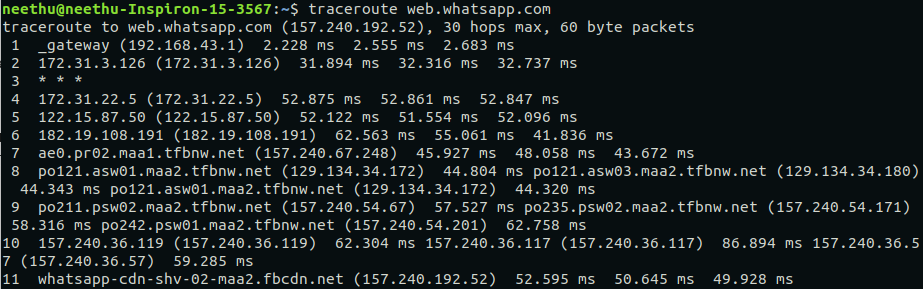
\includegraphics[scale=0.5]{img/e13.png}
        \end{figure}
    \item netstat
        \begin{itemize}
            \item Netstat(Network Statistic) command displays connection info, routing table information etc.
            \item It displays various network related information such as network connections, routing tables, masquerade connections, multicast memberships, interface statistics etc.
        \end{itemize}
        \begin{figure}[h]
            \centering
            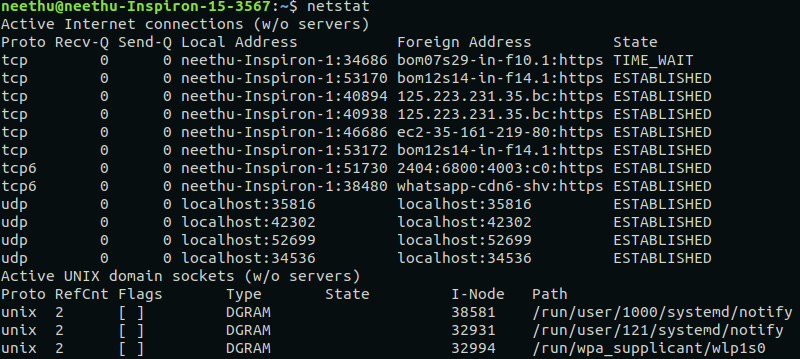
\includegraphics[scale=0.55]{img/e14.png}
        \end{figure}
    \item nslookup
        \begin{itemize}
            \item nslookup is a command-line administrative tool for testing and troubleshooting DNS servers (Domain Name Server).
            \item Most operating systems comes with built-in nslookup feature.
        \end{itemize}
        \begin{figure}[h]
            \centering
            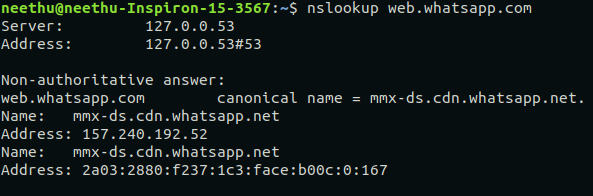
\includegraphics[scale=0.75]{img/e15.png}
        \end{figure}
    \item route
        \begin{itemize}
            \item Its basic function is to show or manipulate IP routing tables.
            \item It can add and delete routes and default Gateway.
        \end{itemize}
        \begin{figure}[h]
            \centering
            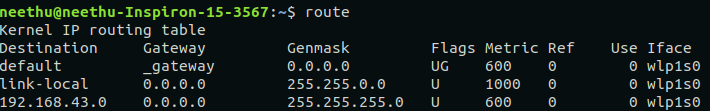
\includegraphics[scale=0.65]{img/e16.png}
        \end{figure}
    \newpage
    \item arp
        \begin{itemize}
            \item It is a protocol used by network nodes to resolve IP addresses to their corresponding MAC addresses.
            \item It can also be used to add an address for which to proxy arp and to forcefully add permanent entries to the ARP table.
        \end{itemize}
        \begin{figure}[h]
            \centering
            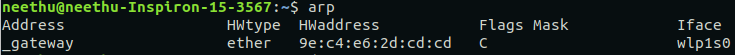
\includegraphics[scale=0.64]{img/e17.png}
        \end{figure}
    \item dig
        \begin{itemize}
            \item Dig (Domain Information Groper) query DNS related information like a record, CNAME, MX Record etc. This command mainly use to troubleshoot DNS related query.
        \end{itemize}
        \begin{figure}[h]
            \centering
            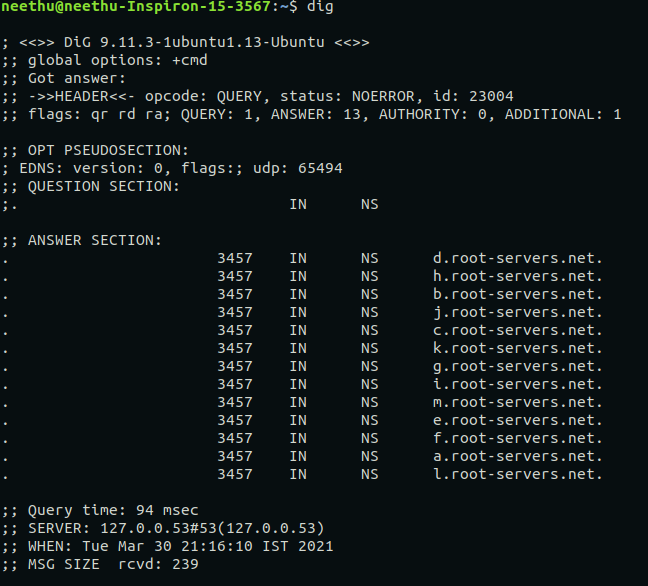
\includegraphics[scale=0.63]{img/e18.png}
        \end{figure}
    \item host
        \begin{itemize}
            \item Host command to find name to IP or IP to name in IPv4 or IPv6 and also query DNS records.
        \end{itemize}
        \begin{figure}[h]
            \centering
            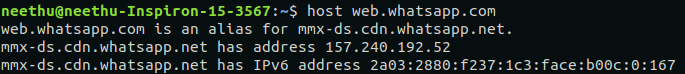
\includegraphics[scale=0.7]{img/e19.png}
        \end{figure}
    \item hostname
        \begin{itemize}
            \item hostname is to identify the host in a network. 
        \end{itemize}
        \begin{figure}[h]
            \centering
            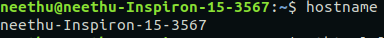
\includegraphics[scale=0.8]{img/e110.png}
        \end{figure}
    \item ethtool
        \begin{itemize}
            \item ethtool is used to view, setting speed and duplex of your Network Interface Card (NIC).
        \end{itemize}
        \begin{figure}[h]
            \centering
            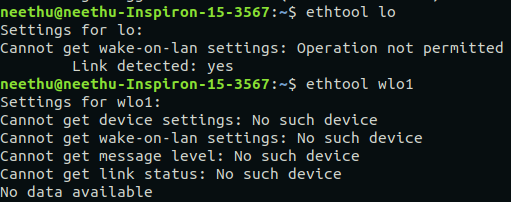
\includegraphics[scale=0.75]{img/e111.png}
        \end{figure}
    
\end{itemize}


\subsection{Result}
Implemented the basic networking commands in Ubuntu 18.04 and the above outputs were obtained.